\documentclass{book}
\usepackage[a4paper,top=2.5cm,bottom=2.5cm,left=2.5cm,right=2.5cm]{geometry}
\usepackage{makeidx}
\usepackage{natbib}
\usepackage{graphicx}
\usepackage{multicol}
\usepackage{float}
\usepackage{listings}
\usepackage{color}
\usepackage{ifthen}
\usepackage[table]{xcolor}
\usepackage{textcomp}
\usepackage{alltt}
\usepackage{ifpdf}
\ifpdf
\usepackage[pdftex,
            pagebackref=true,
            colorlinks=true,
            linkcolor=blue,
            unicode
           ]{hyperref}
\else
\usepackage[ps2pdf,
            pagebackref=true,
            colorlinks=true,
            linkcolor=blue,
            unicode
           ]{hyperref}
\usepackage{pspicture}
\fi
\usepackage[utf8]{inputenc}
\usepackage{mathptmx}
\usepackage[scaled=.90]{helvet}
\usepackage{courier}
\usepackage{sectsty}
\usepackage[titles]{tocloft}
\usepackage{doxygen}
\lstset{language=C++,inputencoding=utf8,basicstyle=\footnotesize,breaklines=true,breakatwhitespace=true,tabsize=8,numbers=left }
\makeindex
\setcounter{tocdepth}{3}
\renewcommand{\footrulewidth}{0.4pt}
\renewcommand{\familydefault}{\sfdefault}
\hfuzz=15pt
\setlength{\emergencystretch}{15pt}
\hbadness=750
\tolerance=750
\begin{document}
\hypersetup{pageanchor=false,citecolor=blue}
\begin{titlepage}
\vspace*{7cm}
\begin{center}
{\Large X\-D\-M\-Lab Project \\[1ex]\large 1.\-1 }\\
\vspace*{1cm}
{\large Generated by Doxygen 1.8.0}\\
\vspace*{0.5cm}
{\small Mon Apr 29 2013 15:11:27}\\
\end{center}
\end{titlepage}
\clearemptydoublepage
\pagenumbering{roman}
\tableofcontents
\clearemptydoublepage
\pagenumbering{arabic}
\hypersetup{pageanchor=true,citecolor=blue}
\chapter{Class Index}
\section{Class Hierarchy}
This inheritance list is sorted roughly, but not completely, alphabetically\-:\begin{DoxyCompactList}
\item \contentsline{section}{X\-:\-:Data$<$ T, N $>$}{\pageref{class_x_1_1_data}}{}
\begin{DoxyCompactList}
\item \contentsline{section}{X\-:\-:Data\-Index1$<$ T, N $>$}{\pageref{class_x_1_1_data_index1}}{}
\end{DoxyCompactList}
\item \contentsline{section}{X\-:\-:Data$<$ T, N1 $\ast$\-N2 $>$}{\pageref{class_x_1_1_data}}{}
\begin{DoxyCompactList}
\item \contentsline{section}{X\-:\-:Data\-Index2$<$ T, N1, N2 $>$}{\pageref{class_x_1_1_data_index2}}{}
\end{DoxyCompactList}
\item \contentsline{section}{X\-:\-:Enumerator1$<$ P1 $>$}{\pageref{class_x_1_1_enumerator1}}{}
\item \contentsline{section}{X\-:\-:Enumerator2$<$ P1, P2 $>$}{\pageref{class_x_1_1_enumerator2}}{}
\item \contentsline{section}{X\-:\-:Index$<$ T $>$}{\pageref{class_x_1_1_index}}{}
\begin{DoxyCompactList}
\item \contentsline{section}{X\-:\-:Index1$<$ T, N $>$}{\pageref{class_x_1_1_index1}}{}
\begin{DoxyCompactList}
\item \contentsline{section}{X\-:\-:Data\-Index1$<$ T, N $>$}{\pageref{class_x_1_1_data_index1}}{}
\end{DoxyCompactList}
\item \contentsline{section}{X\-:\-:Index1$<$ T, N $>$}{\pageref{class_x_1_1_index1}}{}
\begin{DoxyCompactList}
\item \contentsline{section}{X\-:\-:Dataset$<$ T, N $>$}{\pageref{class_x_1_1_dataset}}{}
\end{DoxyCompactList}
\item \contentsline{section}{X\-:\-:Index2$<$ T, N1, N2 $>$}{\pageref{class_x_1_1_index2}}{}
\begin{DoxyCompactList}
\item \contentsline{section}{X\-:\-:Data\-Index2$<$ T, N1, N2 $>$}{\pageref{class_x_1_1_data_index2}}{}
\end{DoxyCompactList}
\end{DoxyCompactList}
\item \contentsline{section}{X\-:\-:Index$<$ D\-T $>$}{\pageref{class_x_1_1_index}}{}
\begin{DoxyCompactList}
\item \contentsline{section}{X\-:\-:Index1$<$ D\-T, N $>$}{\pageref{class_x_1_1_index1}}{}
\begin{DoxyCompactList}
\item \contentsline{section}{X\-:\-:Dataset$<$ D\-T, N $>$}{\pageref{class_x_1_1_dataset}}{}
\begin{DoxyCompactList}
\item \contentsline{section}{X\-:\-:Field$<$ T, 2, P, N $>$}{\pageref{class_x_1_1_field}}{}
\begin{DoxyCompactList}
\item \contentsline{section}{X\-:\-:Field2\-D$<$ T, P1 $\ast$\-P2, N $>$}{\pageref{class_x_1_1_field2_d}}{}
\begin{DoxyCompactList}
\item \contentsline{section}{X\-:\-:Field2\-D\-Index2$<$ T, P1, P2, N $>$}{\pageref{class_x_1_1_field2_d_index2}}{}
\end{DoxyCompactList}
\item \contentsline{section}{X\-:\-:Field2\-D$<$ T, P, N $>$}{\pageref{class_x_1_1_field2_d}}{}
\end{DoxyCompactList}
\item \contentsline{section}{X\-:\-:Field$<$ D\-T, G\-T, P, N $>$}{\pageref{class_x_1_1_field}}{}
\end{DoxyCompactList}
\end{DoxyCompactList}
\end{DoxyCompactList}
\item \contentsline{section}{X\-:\-:Matrix$<$ T, R\-O\-W\-S, C\-O\-L\-S $>$}{\pageref{class_x_1_1_matrix}}{}
\item \contentsline{section}{X\-:\-:Matrix$<$ T, 1, N $>$}{\pageref{class_x_1_1_matrix}}{}
\begin{DoxyCompactList}
\item \contentsline{section}{X\-:\-:Vector$<$ T, N $>$}{\pageref{class_x_1_1_vector}}{}
\end{DoxyCompactList}
\item \contentsline{section}{X\-:\-:Memory}{\pageref{class_x_1_1_memory}}{}
\item \contentsline{section}{X\-:\-:Meshgrid\-Field2\-Filestream$<$ T, P1, P2, N $>$}{\pageref{class_x_1_1_meshgrid_field2_filestream}}{}
\item \contentsline{section}{Normal\-Operation$<$ typename T, xsize N $>$}{\pageref{class_normal_operation_3_01typename_01_t_00_01xsize_01_n_01_4}}{}
\item \contentsline{section}{X\-:\-:x\-Complex$<$ T $>$}{\pageref{class_x_1_1x_complex}}{}
\end{DoxyCompactList}

\chapter{Class Index}
\section{Class List}
Here are the classes, structs, unions and interfaces with brief descriptions\-:\begin{DoxyCompactList}
\item\contentsline{section}{\hyperlink{class_x_1_1_data}{X\-::\-Data$<$ T, N $>$} }{\pageref{class_x_1_1_data}}{}
\item\contentsline{section}{\hyperlink{class_x_1_1_data_index1}{X\-::\-Data\-Index1$<$ T, N $>$} }{\pageref{class_x_1_1_data_index1}}{}
\item\contentsline{section}{\hyperlink{class_x_1_1_data_index2}{X\-::\-Data\-Index2$<$ T, N1, N2 $>$} }{\pageref{class_x_1_1_data_index2}}{}
\item\contentsline{section}{\hyperlink{class_x_1_1_dataset}{X\-::\-Dataset$<$ D\-T, N $>$} }{\pageref{class_x_1_1_dataset}}{}
\item\contentsline{section}{\hyperlink{class_x_1_1_enumerator1}{X\-::\-Enumerator1$<$ P1 $>$} }{\pageref{class_x_1_1_enumerator1}}{}
\item\contentsline{section}{\hyperlink{class_x_1_1_enumerator2}{X\-::\-Enumerator2$<$ P1, P2 $>$} }{\pageref{class_x_1_1_enumerator2}}{}
\item\contentsline{section}{\hyperlink{class_x_1_1_field}{X\-::\-Field$<$ D\-T, G\-T, P, N $>$} }{\pageref{class_x_1_1_field}}{}
\item\contentsline{section}{\hyperlink{class_x_1_1_field2_d}{X\-::\-Field2\-D$<$ T, P, N $>$} }{\pageref{class_x_1_1_field2_d}}{}
\item\contentsline{section}{\hyperlink{class_x_1_1_field2_d_index2}{X\-::\-Field2\-D\-Index2$<$ T, P1, P2, N $>$} }{\pageref{class_x_1_1_field2_d_index2}}{}
\item\contentsline{section}{\hyperlink{class_x_1_1_index}{X\-::\-Index$<$ T $>$} }{\pageref{class_x_1_1_index}}{}
\item\contentsline{section}{\hyperlink{class_x_1_1_index1}{X\-::\-Index1$<$ T, N $>$} }{\pageref{class_x_1_1_index1}}{}
\item\contentsline{section}{\hyperlink{class_x_1_1_index2}{X\-::\-Index2$<$ T, N1, N2 $>$} }{\pageref{class_x_1_1_index2}}{}
\item\contentsline{section}{\hyperlink{class_x_1_1_matrix}{X\-::\-Matrix$<$ T, R\-O\-W\-S, C\-O\-L\-S $>$} }{\pageref{class_x_1_1_matrix}}{}
\item\contentsline{section}{\hyperlink{class_x_1_1_memory}{X\-::\-Memory} }{\pageref{class_x_1_1_memory}}{}
\item\contentsline{section}{\hyperlink{class_x_1_1_meshgrid_field2_filestream}{X\-::\-Meshgrid\-Field2\-Filestream$<$ T, P1, P2, N $>$} }{\pageref{class_x_1_1_meshgrid_field2_filestream}}{}
\item\contentsline{section}{\hyperlink{class_normal_operation_3_01typename_01_t_00_01xsize_01_n_01_4}{Normal\-Operation$<$ typename T, xsize N $>$} }{\pageref{class_normal_operation_3_01typename_01_t_00_01xsize_01_n_01_4}}{}
\item\contentsline{section}{\hyperlink{class_x_1_1_vector}{X\-::\-Vector$<$ T, N $>$} }{\pageref{class_x_1_1_vector}}{}
\item\contentsline{section}{\hyperlink{class_x_1_1x_complex}{X\-::x\-Complex$<$ T $>$} }{\pageref{class_x_1_1x_complex}}{}
\end{DoxyCompactList}

\chapter{Class Documentation}
\hypertarget{class_x_1_1_data}{\section{X\-:\-:Data$<$ T, N $>$ Class Template Reference}
\label{class_x_1_1_data}\index{X\-::\-Data$<$ T, N $>$@{X\-::\-Data$<$ T, N $>$}}
}


This class is the base class for all the data.  




{\ttfamily \#include $<$data.\-h$>$}

Inheritance diagram for X\-:\-:Data$<$ T, N $>$\-:\begin{figure}[H]
\begin{center}
\leavevmode
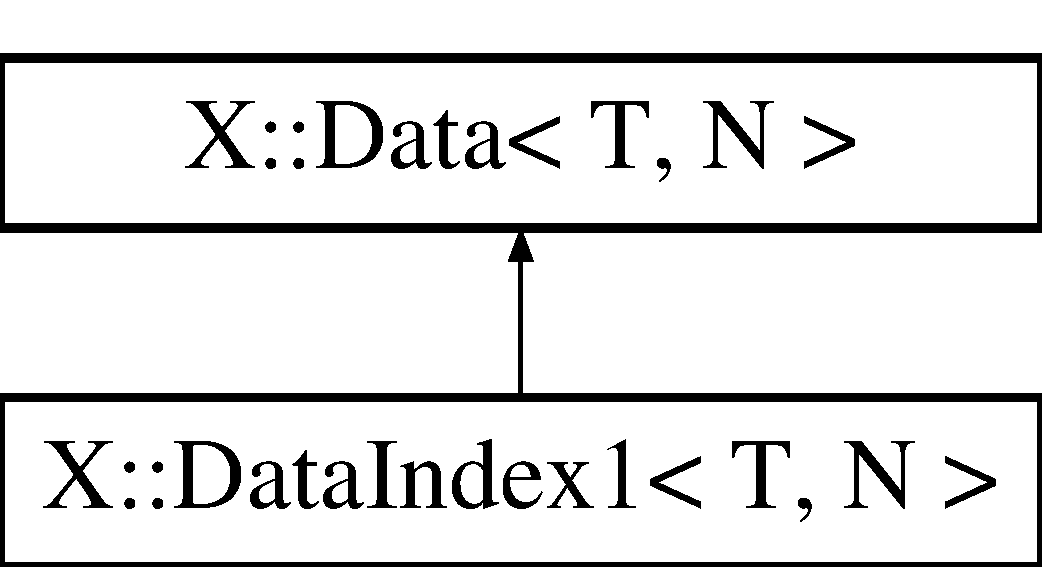
\includegraphics[height=2.000000cm]{class_x_1_1_data}
\end{center}
\end{figure}
\subsection*{Public Member Functions}
\begin{DoxyCompactItemize}
\item 
\hyperlink{class_x_1_1_data_a9ad5f351292008abe819ecaad1e3c94d}{Data} ()
\item 
\hyperlink{class_x_1_1_data_a2b21e425670199f07a7e264b24f69214}{$\sim$\-Data} ()
\item 
T $\ast$ \hyperlink{class_x_1_1_data_a085e20937e473698958910dfe31780aa}{get\-Data\-Pointer} ()
\item 
T $\ast$ \hyperlink{class_x_1_1_data_ac3fd035b3814e662ef527a00034f947d}{p} ()
\item 
T \& \hyperlink{class_x_1_1_data_a9a0a3e674daebe2750d8d7f233e7d0ce}{get\-Data} (xsize i)
\item 
void \hyperlink{class_x_1_1_data_ac9e98c6fbdfdd23b664e6ac610fd672a}{copy\-Data} (\hyperlink{class_x_1_1_data}{Data}$<$ T, N $>$ \&data)
\item 
\hypertarget{class_x_1_1_data_a8c1665070bafded63fcd3bc3f7afbff2}{void {\bfseries operator+=} (\hyperlink{class_x_1_1_data}{Data}$<$ T, N $>$ \&B)}\label{class_x_1_1_data_a8c1665070bafded63fcd3bc3f7afbff2}

\item 
\hypertarget{class_x_1_1_data_a53b2f3843000d2f71386a02644e40784}{{\footnotesize template$<$typename B $>$ }\\void {\bfseries operator+=} (B b)}\label{class_x_1_1_data_a53b2f3843000d2f71386a02644e40784}

\item 
\hypertarget{class_x_1_1_data_a9dd49ecafa28bec173a1d5af0fee2a3e}{void {\bfseries operator-\/=} (\hyperlink{class_x_1_1_data}{Data}$<$ T, N $>$ \&B)}\label{class_x_1_1_data_a9dd49ecafa28bec173a1d5af0fee2a3e}

\item 
\hypertarget{class_x_1_1_data_a153fccaadec2bf9da88caa7e31b8a3f5}{{\footnotesize template$<$typename B $>$ }\\void {\bfseries operator-\/=} (B b)}\label{class_x_1_1_data_a153fccaadec2bf9da88caa7e31b8a3f5}

\item 
\hypertarget{class_x_1_1_data_a837aad97f0179a95de5c768e19ce9272}{void {\bfseries operator$\ast$=} (\hyperlink{class_x_1_1_data}{Data}$<$ T, N $>$ \&B)}\label{class_x_1_1_data_a837aad97f0179a95de5c768e19ce9272}

\item 
\hypertarget{class_x_1_1_data_a3460e08914f4d7337ae106c291cf6818}{{\footnotesize template$<$typename B $>$ }\\void {\bfseries operator$\ast$=} (B b)}\label{class_x_1_1_data_a3460e08914f4d7337ae106c291cf6818}

\item 
\hypertarget{class_x_1_1_data_a3279d56933969537c5f12ff0a60c55a1}{void {\bfseries operator/=} (\hyperlink{class_x_1_1_data}{Data}$<$ T, N $>$ \&B)}\label{class_x_1_1_data_a3279d56933969537c5f12ff0a60c55a1}

\item 
\hypertarget{class_x_1_1_data_a78a26985cb6596c9d9e475f54887bbe3}{{\footnotesize template$<$typename B $>$ }\\void {\bfseries operator/=} (B b)}\label{class_x_1_1_data_a78a26985cb6596c9d9e475f54887bbe3}

\end{DoxyCompactItemize}


\subsection{Detailed Description}
\subsubsection*{template$<$typename T, xsize N$>$class X\-::\-Data$<$ T, N $>$}

This class is the base class for all the data. 

\begin{DoxyAuthor}{Author}
Hsu, Tien-\/\-Yiao 
\end{DoxyAuthor}
\begin{DoxyCopyright}{Copyright}
N\-T\-U\-A\-S D\-M\-Lab 
\end{DoxyCopyright}
\begin{DoxyDate}{Date}
2013/04/27 
\end{DoxyDate}
\begin{DoxyVersion}{Version}
1.\-0
\end{DoxyVersion}
\hyperlink{class_x_1_1_data}{Data} needs to be specified its data type and number of elements. \#data 

\subsection{Constructor \& Destructor Documentation}
\hypertarget{class_x_1_1_data_a9ad5f351292008abe819ecaad1e3c94d}{\index{X\-::\-Data@{X\-::\-Data}!Data@{Data}}
\index{Data@{Data}!X::Data@{X\-::\-Data}}
\subsubsection[{Data}]{\setlength{\rightskip}{0pt plus 5cm}template$<$typename T, xsize N$>$ {\bf X\-::\-Data}$<$ T, N $>$\-::{\bf Data} (
\begin{DoxyParamCaption}
{}
\end{DoxyParamCaption}
)}}\label{class_x_1_1_data_a9ad5f351292008abe819ecaad1e3c94d}
Initialize an array of N elements with type T. They are all with default initialized value. \hypertarget{class_x_1_1_data_a2b21e425670199f07a7e264b24f69214}{\index{X\-::\-Data@{X\-::\-Data}!$\sim$\-Data@{$\sim$\-Data}}
\index{$\sim$\-Data@{$\sim$\-Data}!X::Data@{X\-::\-Data}}
\subsubsection[{$\sim$\-Data}]{\setlength{\rightskip}{0pt plus 5cm}template$<$typename T, xsize N$>$ {\bf X\-::\-Data}$<$ T, N $>$\-::$\sim${\bf Data} (
\begin{DoxyParamCaption}
{}
\end{DoxyParamCaption}
)}}\label{class_x_1_1_data_a2b21e425670199f07a7e264b24f69214}
Deconstructor frees all the heap memory of the object. 

\subsection{Member Function Documentation}
\hypertarget{class_x_1_1_data_ac9e98c6fbdfdd23b664e6ac610fd672a}{\index{X\-::\-Data@{X\-::\-Data}!copy\-Data@{copy\-Data}}
\index{copy\-Data@{copy\-Data}!X::Data@{X\-::\-Data}}
\subsubsection[{copy\-Data}]{\setlength{\rightskip}{0pt plus 5cm}template$<$typename T, xsize N$>$ void {\bf X\-::\-Data}$<$ T, N $>$\-::{\bf copy\-Data} (
\begin{DoxyParamCaption}
\item[{{\bf Data}$<$ T, N $>$ \&}]{data}
\end{DoxyParamCaption}
)\hspace{0.3cm}{\ttfamily  \mbox{[}inline\mbox{]}}}}\label{class_x_1_1_data_ac9e98c6fbdfdd23b664e6ac610fd672a}
Copies the value of another data. \hypertarget{class_x_1_1_data_a9a0a3e674daebe2750d8d7f233e7d0ce}{\index{X\-::\-Data@{X\-::\-Data}!get\-Data@{get\-Data}}
\index{get\-Data@{get\-Data}!X::Data@{X\-::\-Data}}
\subsubsection[{get\-Data}]{\setlength{\rightskip}{0pt plus 5cm}template$<$typename T, xsize N$>$ T\& {\bf X\-::\-Data}$<$ T, N $>$\-::{\bf get\-Data} (
\begin{DoxyParamCaption}
\item[{xsize}]{i}
\end{DoxyParamCaption}
)\hspace{0.3cm}{\ttfamily  \mbox{[}inline\mbox{]}}}}\label{class_x_1_1_data_a9a0a3e674daebe2750d8d7f233e7d0ce}
Get the i-\/th element of the data. \hypertarget{class_x_1_1_data_a085e20937e473698958910dfe31780aa}{\index{X\-::\-Data@{X\-::\-Data}!get\-Data\-Pointer@{get\-Data\-Pointer}}
\index{get\-Data\-Pointer@{get\-Data\-Pointer}!X::Data@{X\-::\-Data}}
\subsubsection[{get\-Data\-Pointer}]{\setlength{\rightskip}{0pt plus 5cm}template$<$typename T, xsize N$>$ T$\ast$ {\bf X\-::\-Data}$<$ T, N $>$\-::{\bf get\-Data\-Pointer} (
\begin{DoxyParamCaption}
{}
\end{DoxyParamCaption}
)\hspace{0.3cm}{\ttfamily  \mbox{[}inline\mbox{]}}}}\label{class_x_1_1_data_a085e20937e473698958910dfe31780aa}
Return the pointer of the data \hypertarget{class_x_1_1_data_ac3fd035b3814e662ef527a00034f947d}{\index{X\-::\-Data@{X\-::\-Data}!p@{p}}
\index{p@{p}!X::Data@{X\-::\-Data}}
\subsubsection[{p}]{\setlength{\rightskip}{0pt plus 5cm}template$<$typename T, xsize N$>$ T$\ast$ {\bf X\-::\-Data}$<$ T, N $>$\-::{\bf p} (
\begin{DoxyParamCaption}
{}
\end{DoxyParamCaption}
)\hspace{0.3cm}{\ttfamily  \mbox{[}inline\mbox{]}}}}\label{class_x_1_1_data_ac3fd035b3814e662ef527a00034f947d}
Abbreviation for \hyperlink{class_x_1_1_data_a085e20937e473698958910dfe31780aa}{get\-Data\-Pointer()} 

The documentation for this class was generated from the following file\-:\begin{DoxyCompactItemize}
\item 
src/data.\-h\end{DoxyCompactItemize}

\hypertarget{class_x_1_1_data_index1}{\section{X\-:\-:Data\-Index1$<$ T, N $>$ Class Template Reference}
\label{class_x_1_1_data_index1}\index{X\-::\-Data\-Index1$<$ T, N $>$@{X\-::\-Data\-Index1$<$ T, N $>$}}
}


This class is for 1-\/dimensional data.  




{\ttfamily \#include $<$data\-\_\-index\-\_\-1.\-h$>$}

Inheritance diagram for X\-:\-:Data\-Index1$<$ T, N $>$\-:\begin{figure}[H]
\begin{center}
\leavevmode
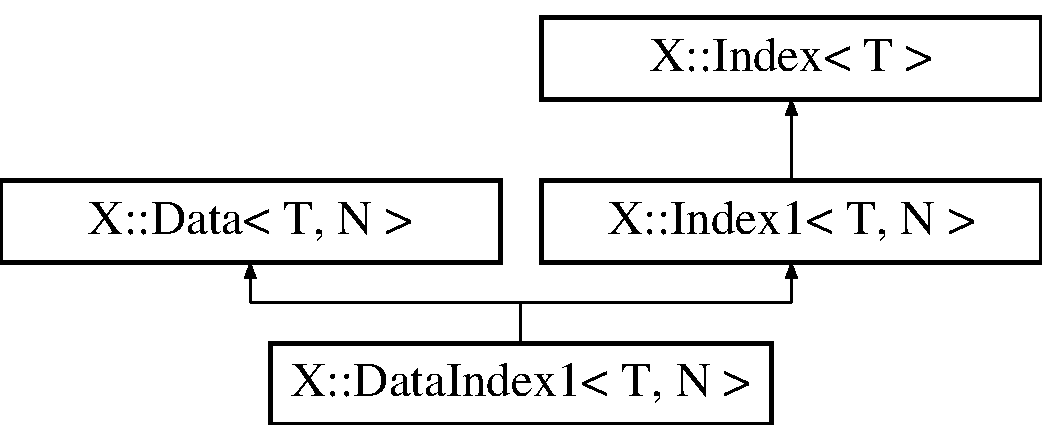
\includegraphics[height=3.000000cm]{class_x_1_1_data_index1}
\end{center}
\end{figure}
\subsection*{Public Member Functions}
\begin{DoxyCompactItemize}
\item 
\hypertarget{class_x_1_1_data_index1_a2943aafc09d6e22164a2ec424ecc326a}{{\bfseries Data\-Index1} (T $\ast$)}\label{class_x_1_1_data_index1_a2943aafc09d6e22164a2ec424ecc326a}

\end{DoxyCompactItemize}


\subsection{Detailed Description}
\subsubsection*{template$<$typename T, xsize N$>$class X\-::\-Data\-Index1$<$ T, N $>$}

This class is for 1-\/dimensional data. 

\begin{DoxyAuthor}{Author}
Hsu, Tien-\/\-Yiao 
\end{DoxyAuthor}
\begin{DoxyCopyright}{Copyright}
N\-T\-U\-A\-S D\-M\-Lab 
\end{DoxyCopyright}
\begin{DoxyDate}{Date}
2013/04/29 
\end{DoxyDate}
\begin{DoxyVersion}{Version}
1.\-0 
\end{DoxyVersion}


The documentation for this class was generated from the following file\-:\begin{DoxyCompactItemize}
\item 
src/data\-\_\-index\-\_\-1.\-h\end{DoxyCompactItemize}

\hypertarget{class_x_1_1_data_index2}{\section{X\-:\-:Data\-Index2$<$ T, N1, N2 $>$ Class Template Reference}
\label{class_x_1_1_data_index2}\index{X\-::\-Data\-Index2$<$ T, N1, N2 $>$@{X\-::\-Data\-Index2$<$ T, N1, N2 $>$}}
}
Inheritance diagram for X\-:\-:Data\-Index2$<$ T, N1, N2 $>$\-:\begin{figure}[H]
\begin{center}
\leavevmode
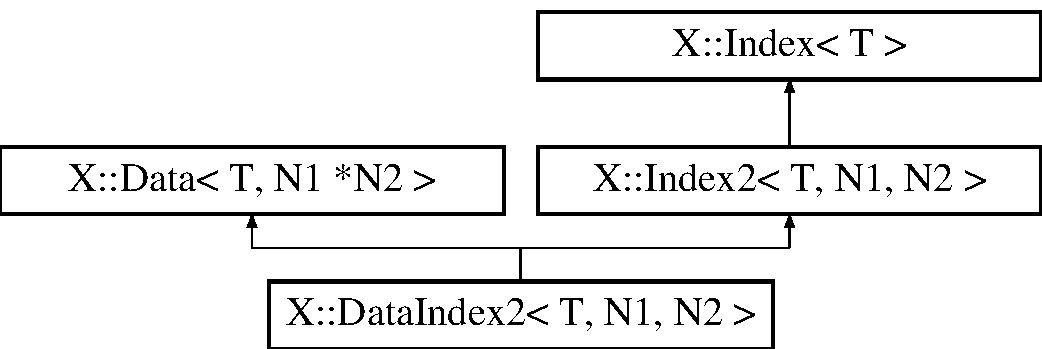
\includegraphics[height=3.000000cm]{class_x_1_1_data_index2}
\end{center}
\end{figure}
\subsection*{Public Member Functions}
\begin{DoxyCompactItemize}
\item 
\hypertarget{class_x_1_1_data_index2_a25805f76116adcea21754503f42ac30f}{void {\bfseries Default\-Constructor} ()}\label{class_x_1_1_data_index2_a25805f76116adcea21754503f42ac30f}

\item 
\hypertarget{class_x_1_1_data_index2_a23b362365b1115b5e922ee50ca026c28}{{\bfseries Data\-Index2} (T $\ast$)}\label{class_x_1_1_data_index2_a23b362365b1115b5e922ee50ca026c28}

\end{DoxyCompactItemize}
\subsubsection*{template$<$typename T, xsize N1, xsize N2$>$ class X\-::\-Data\-Index2$<$ T, N1, N2 $>$}



The documentation for this class was generated from the following file\-:\begin{DoxyCompactItemize}
\item 
src/data\-\_\-index\-\_\-2.\-h\end{DoxyCompactItemize}

\hypertarget{class_x_1_1_dataset}{\section{X\-:\-:Dataset$<$ D\-T, N $>$ Class Template Reference}
\label{class_x_1_1_dataset}\index{X\-::\-Dataset$<$ D\-T, N $>$@{X\-::\-Dataset$<$ D\-T, N $>$}}
}
Inheritance diagram for X\-:\-:Dataset$<$ D\-T, N $>$\-:\begin{figure}[H]
\begin{center}
\leavevmode
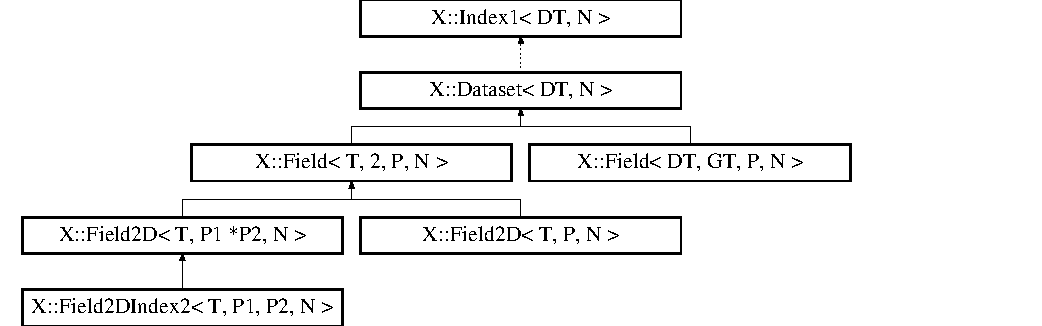
\includegraphics[height=4.381846cm]{class_x_1_1_dataset}
\end{center}
\end{figure}
\subsubsection*{template$<$typename D\-T, xsize N$>$ class X\-::\-Dataset$<$ D\-T, N $>$}



The documentation for this class was generated from the following file\-:\begin{DoxyCompactItemize}
\item 
src/dataset.\-h\end{DoxyCompactItemize}

\hypertarget{class_x_1_1_enumerator1}{\section{X\-:\-:Enumerator1$<$ P1 $>$ Class Template Reference}
\label{class_x_1_1_enumerator1}\index{X\-::\-Enumerator1$<$ P1 $>$@{X\-::\-Enumerator1$<$ P1 $>$}}
}
\subsection*{Public Member Functions}
\begin{DoxyCompactItemize}
\item 
\hypertarget{class_x_1_1_enumerator1_ab9ac1342d0ad82b938afa6daa705bafc}{{\footnotesize template$<$typename Fn $>$ }\\void {\bfseries each\-\_\-index} (Fn f) const }\label{class_x_1_1_enumerator1_ab9ac1342d0ad82b938afa6daa705bafc}

\end{DoxyCompactItemize}
\subsubsection*{template$<$xsize P1$>$ class X\-::\-Enumerator1$<$ P1 $>$}



The documentation for this class was generated from the following file\-:\begin{DoxyCompactItemize}
\item 
src/enumerator.\-h\end{DoxyCompactItemize}

\hypertarget{class_x_1_1_enumerator2}{\section{X\-:\-:Enumerator2$<$ P1, P2 $>$ Class Template Reference}
\label{class_x_1_1_enumerator2}\index{X\-::\-Enumerator2$<$ P1, P2 $>$@{X\-::\-Enumerator2$<$ P1, P2 $>$}}
}
\subsection*{Public Member Functions}
\begin{DoxyCompactItemize}
\item 
\hypertarget{class_x_1_1_enumerator2_a5d834fbc808b8429dfe749133a856f2c}{{\footnotesize template$<$typename Fn $>$ }\\void {\bfseries each\-\_\-index} (Fn f) const }\label{class_x_1_1_enumerator2_a5d834fbc808b8429dfe749133a856f2c}

\end{DoxyCompactItemize}
\subsubsection*{template$<$xsize P1, xsize P2$>$ class X\-::\-Enumerator2$<$ P1, P2 $>$}



The documentation for this class was generated from the following file\-:\begin{DoxyCompactItemize}
\item 
src/enumerator.\-h\end{DoxyCompactItemize}

\hypertarget{class_x_1_1_field}{\section{X\-:\-:Field$<$ D\-T, G\-T, P, N $>$ Class Template Reference}
\label{class_x_1_1_field}\index{X\-::\-Field$<$ D\-T, G\-T, P, N $>$@{X\-::\-Field$<$ D\-T, G\-T, P, N $>$}}
}
Inheritance diagram for X\-:\-:Field$<$ D\-T, G\-T, P, N $>$\-:\begin{figure}[H]
\begin{center}
\leavevmode
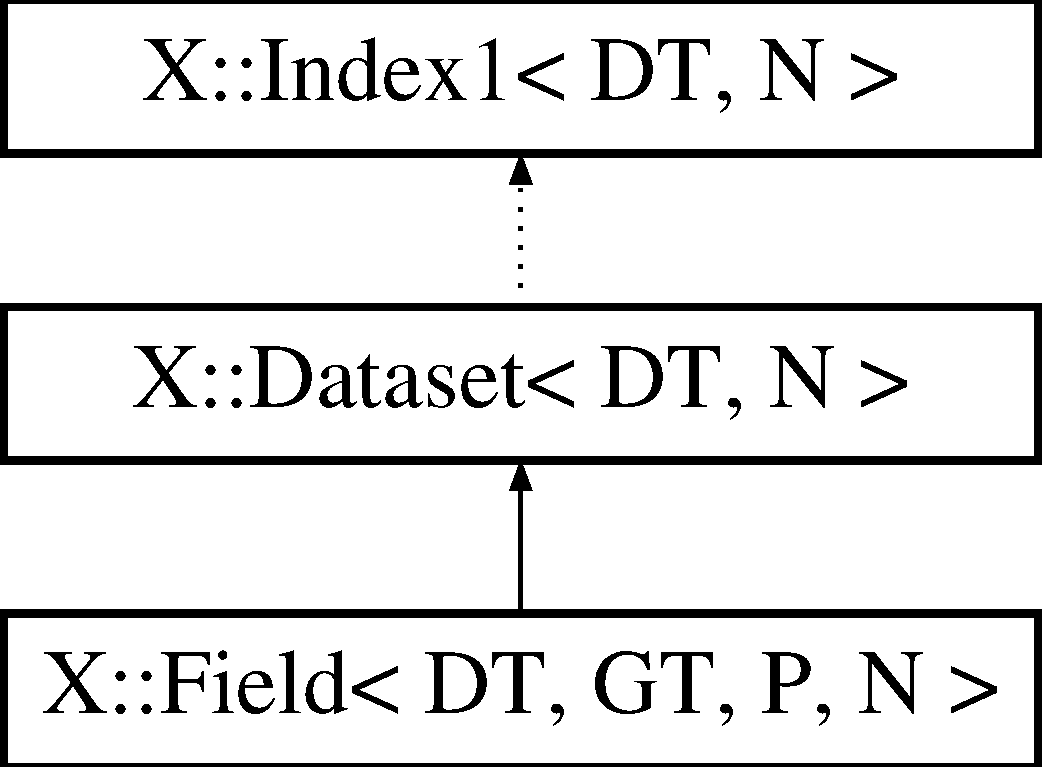
\includegraphics[height=3.000000cm]{class_x_1_1_field}
\end{center}
\end{figure}
\subsection*{Public Member Functions}
\begin{DoxyCompactItemize}
\item 
\hypertarget{class_x_1_1_field_a0308f8c4bc709dd9075bc6b246298604}{G\-T \& {\bfseries get\-Grid} ()}\label{class_x_1_1_field_a0308f8c4bc709dd9075bc6b246298604}

\end{DoxyCompactItemize}
\subsubsection*{template$<$typename D\-T, typename G\-T, xsize P, xsize N$>$ class X\-::\-Field$<$ D\-T, G\-T, P, N $>$}



The documentation for this class was generated from the following file\-:\begin{DoxyCompactItemize}
\item 
src/field.\-h\end{DoxyCompactItemize}

\hypertarget{class_x_1_1_field2_d}{\section{X\-:\-:Field2\-D$<$ T, P, N $>$ Class Template Reference}
\label{class_x_1_1_field2_d}\index{X\-::\-Field2\-D$<$ T, P, N $>$@{X\-::\-Field2\-D$<$ T, P, N $>$}}
}
Inheritance diagram for X\-:\-:Field2\-D$<$ T, P, N $>$\-:\begin{figure}[H]
\begin{center}
\leavevmode
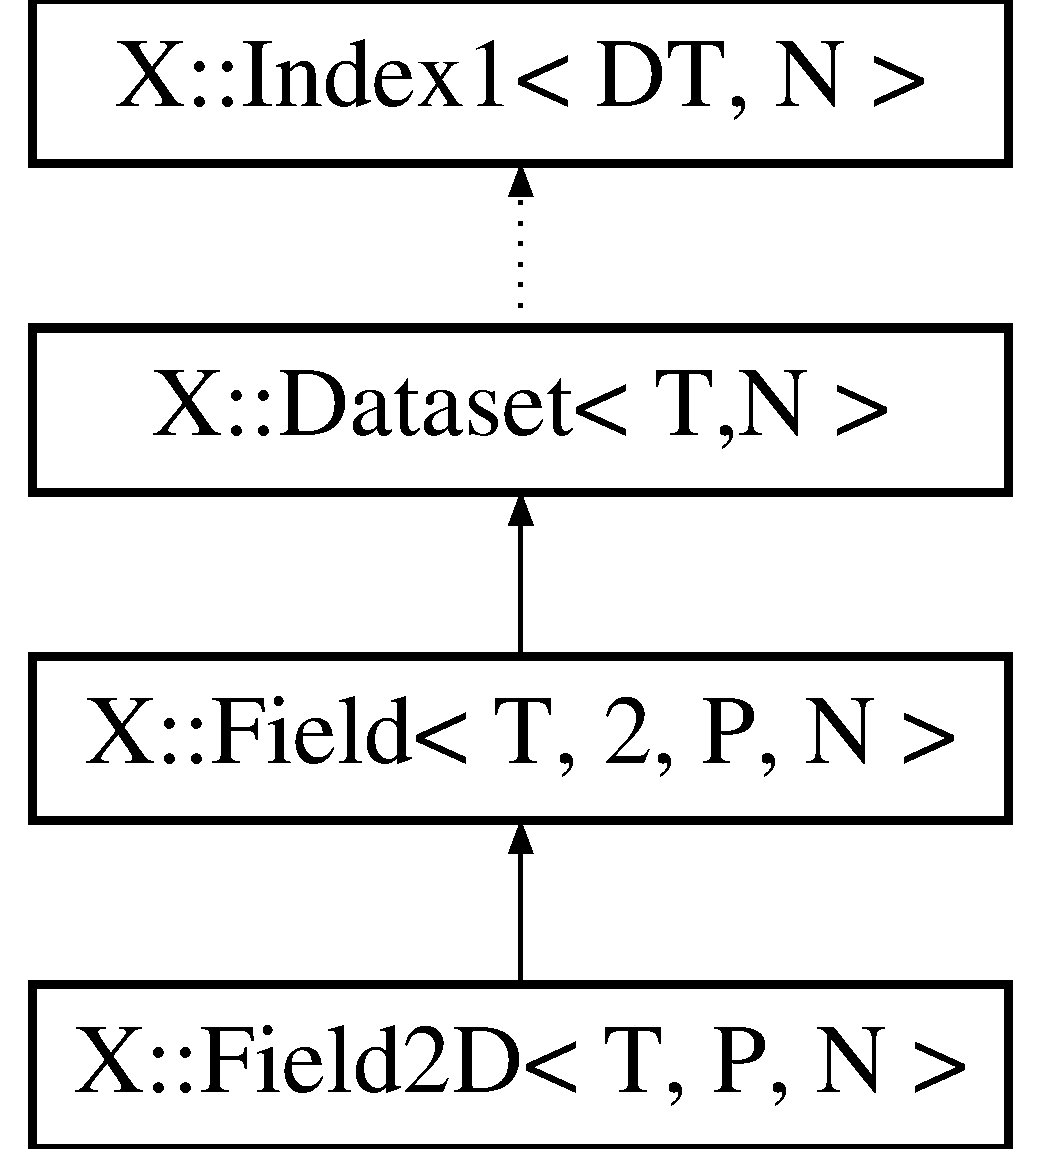
\includegraphics[height=4.000000cm]{class_x_1_1_field2_d}
\end{center}
\end{figure}
\subsubsection*{template$<$typename T, xsize P, xsize N$>$ class X\-::\-Field2\-D$<$ T, P, N $>$}



The documentation for this class was generated from the following file\-:\begin{DoxyCompactItemize}
\item 
src/field2d.\-h\end{DoxyCompactItemize}

\hypertarget{class_x_1_1_field2_d_index2}{\section{X\-:\-:Field2\-D\-Index2$<$ T, P1, P2, N $>$ Class Template Reference}
\label{class_x_1_1_field2_d_index2}\index{X\-::\-Field2\-D\-Index2$<$ T, P1, P2, N $>$@{X\-::\-Field2\-D\-Index2$<$ T, P1, P2, N $>$}}
}
Inheritance diagram for X\-:\-:Field2\-D\-Index2$<$ T, P1, P2, N $>$\-:\begin{figure}[H]
\begin{center}
\leavevmode
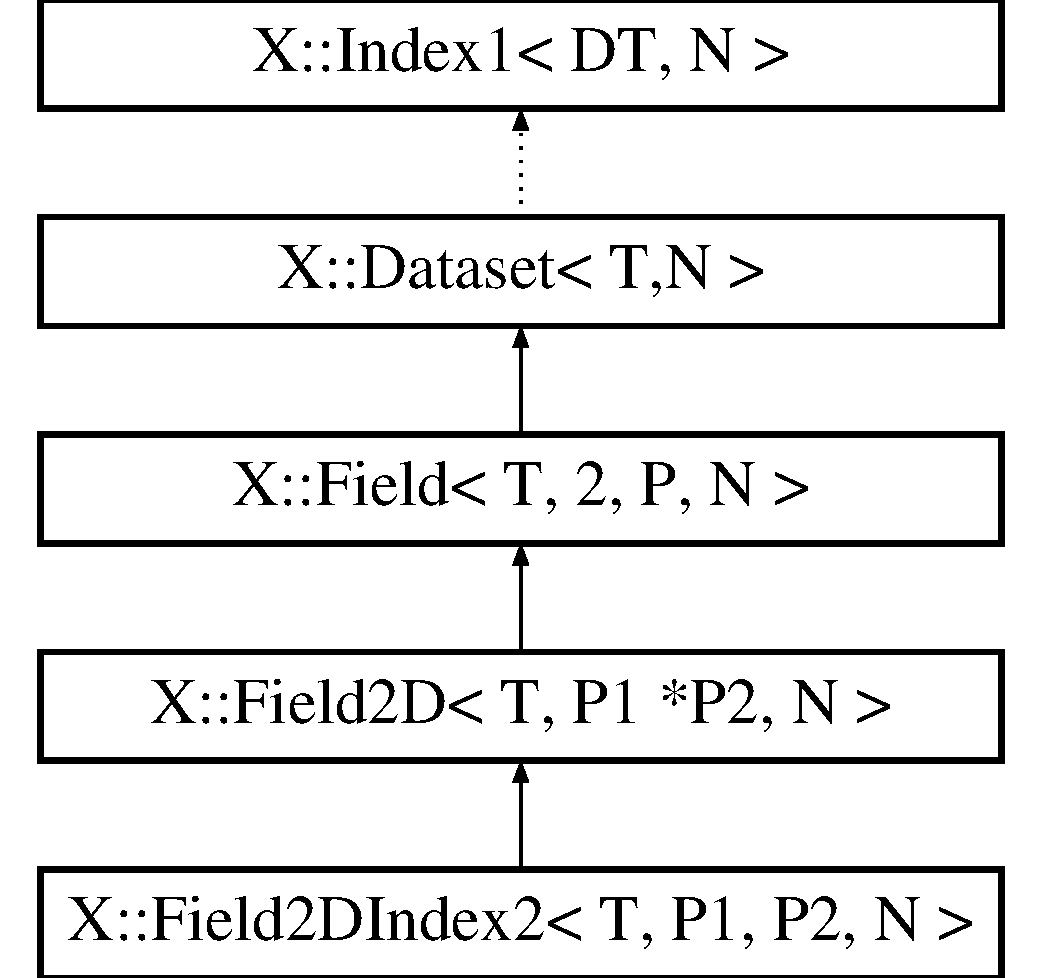
\includegraphics[height=5.000000cm]{class_x_1_1_field2_d_index2}
\end{center}
\end{figure}
\subsection*{Public Member Functions}
\begin{DoxyCompactItemize}
\item 
\hypertarget{class_x_1_1_field2_d_index2_a30fbc232fc63fe00db749020e19e1230}{T \& {\bfseries operator()} (xsize n, xsize i, xsize j)}\label{class_x_1_1_field2_d_index2_a30fbc232fc63fe00db749020e19e1230}

\end{DoxyCompactItemize}
\subsubsection*{template$<$typename T, xsize P1, xsize P2, xsize N$>$ class X\-::\-Field2\-D\-Index2$<$ T, P1, P2, N $>$}



The documentation for this class was generated from the following file\-:\begin{DoxyCompactItemize}
\item 
src/field2dindex2.\-h\end{DoxyCompactItemize}

\hypertarget{class_x_1_1_index}{\section{X\-:\-:Index$<$ T $>$ Class Template Reference}
\label{class_x_1_1_index}\index{X\-::\-Index$<$ T $>$@{X\-::\-Index$<$ T $>$}}
}


This class is the base class for all the \hyperlink{class_x_1_1_index}{Index}. \hyperlink{class_x_1_1_data}{Data} is an 1-\/dimensional array of data, while sometimes we need more than 1 index. Programmers may derived from this class to have their own way to access data.  




{\ttfamily \#include $<$index.\-h$>$}

Inheritance diagram for X\-:\-:Index$<$ T $>$\-:\begin{figure}[H]
\begin{center}
\leavevmode
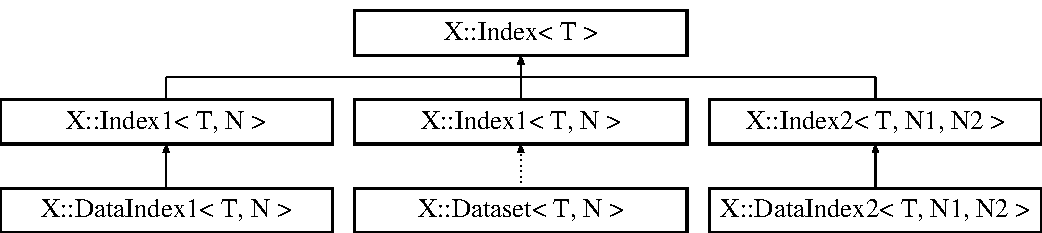
\includegraphics[height=3.000000cm]{class_x_1_1_index}
\end{center}
\end{figure}
\subsection*{Public Member Functions}
\begin{DoxyCompactItemize}
\item 
\hypertarget{class_x_1_1_index_aa61272169a7dd0ab80ea7a7de771c62e}{T $\ast$ {\bfseries get\-Target\-Data\-Pointer} ()}\label{class_x_1_1_index_aa61272169a7dd0ab80ea7a7de771c62e}

\item 
\hypertarget{class_x_1_1_index_a1de180b669777c349047cb3ec10cca48}{void {\bfseries set\-Target\-Data\-Pointer} (T $\ast$data)}\label{class_x_1_1_index_a1de180b669777c349047cb3ec10cca48}

\end{DoxyCompactItemize}


\subsection{Detailed Description}
\subsubsection*{template$<$typename T$>$class X\-::\-Index$<$ T $>$}

This class is the base class for all the \hyperlink{class_x_1_1_index}{Index}. \hyperlink{class_x_1_1_data}{Data} is an 1-\/dimensional array of data, while sometimes we need more than 1 index. Programmers may derived from this class to have their own way to access data. 

\begin{DoxyAuthor}{Author}
Hsu, Tien-\/\-Yiao 
\end{DoxyAuthor}
\begin{DoxyCopyright}{Copyright}
N\-T\-U\-A\-S D\-M\-Lab 
\end{DoxyCopyright}
\begin{DoxyDate}{Date}
2013/04/27 
\end{DoxyDate}
\begin{DoxyVersion}{Version}
1.\-0 
\end{DoxyVersion}


The documentation for this class was generated from the following file\-:\begin{DoxyCompactItemize}
\item 
src/index.\-h\end{DoxyCompactItemize}

\hypertarget{class_x_1_1_index1}{\section{X\-:\-:Index1$<$ T, N $>$ Class Template Reference}
\label{class_x_1_1_index1}\index{X\-::\-Index1$<$ T, N $>$@{X\-::\-Index1$<$ T, N $>$}}
}


This class is the class for 1-\/dimensional index.  




{\ttfamily \#include $<$index\-\_\-1.\-h$>$}

Inheritance diagram for X\-:\-:Index1$<$ T, N $>$\-:\begin{figure}[H]
\begin{center}
\leavevmode
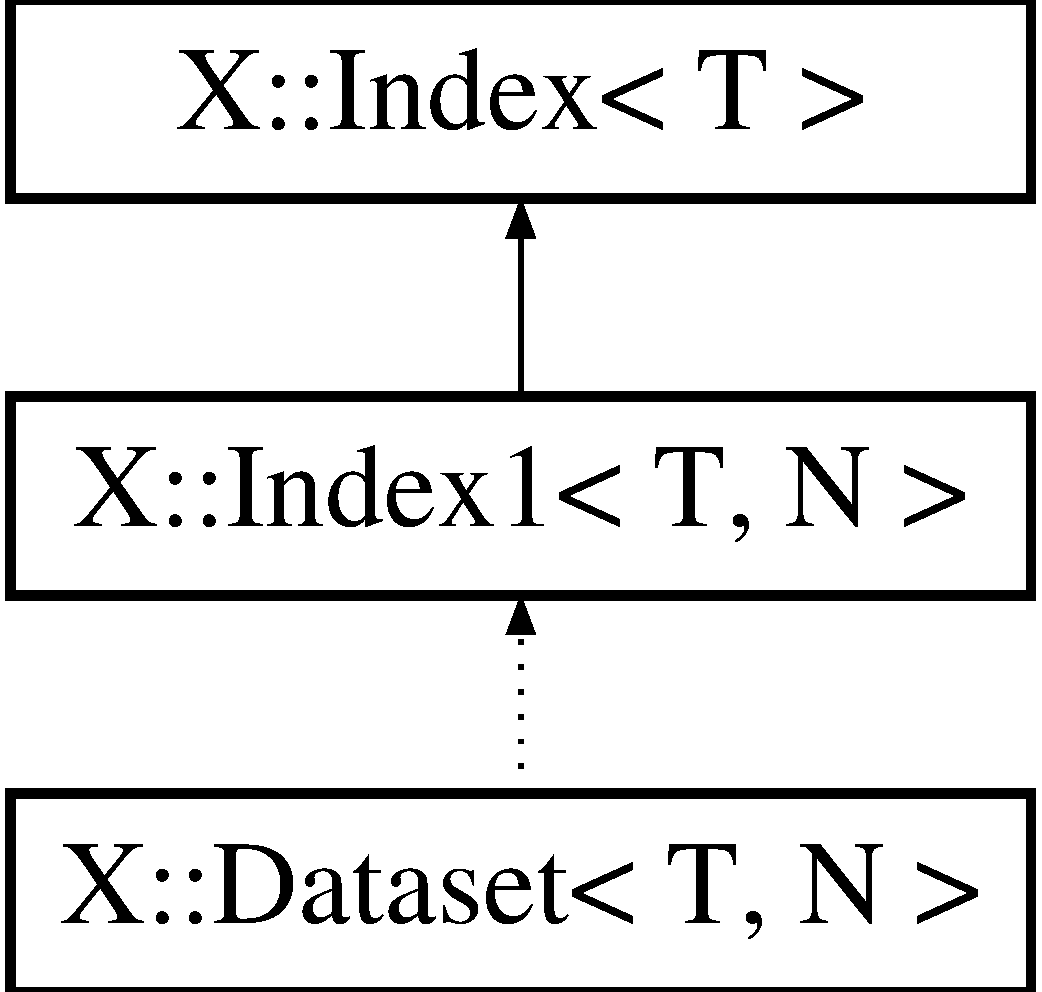
\includegraphics[height=3.000000cm]{class_x_1_1_index1}
\end{center}
\end{figure}
\subsection*{Public Member Functions}
\begin{DoxyCompactItemize}
\item 
\hypertarget{class_x_1_1_index1_a1a3384046f034e8c7abb66f33e06872d}{{\bfseries Index1} (T $\ast$data)}\label{class_x_1_1_index1_a1a3384046f034e8c7abb66f33e06872d}

\item 
virtual T \& \hyperlink{class_x_1_1_index1_a2d876d68fd4b7248660909862d2fd66b}{operator()} (xsize i)
\item 
virtual T \& \hyperlink{class_x_1_1_index1_af340b1faa1a33473a9a1f972e1a2f7a1}{operator\mbox{[}$\,$\mbox{]}} (xsize i)
\end{DoxyCompactItemize}


\subsection{Detailed Description}
\subsubsection*{template$<$typename T, xsize N$>$class X\-::\-Index1$<$ T, N $>$}

This class is the class for 1-\/dimensional index. 

\begin{DoxyAuthor}{Author}
Hsu, Tien-\/\-Yiao 
\end{DoxyAuthor}
\begin{DoxyCopyright}{Copyright}
N\-T\-U\-A\-S D\-M\-Lab 
\end{DoxyCopyright}
\begin{DoxyDate}{Date}
2013/04/27 
\end{DoxyDate}
\begin{DoxyVersion}{Version}
1.\-0 
\end{DoxyVersion}


\subsection{Member Function Documentation}
\hypertarget{class_x_1_1_index1_a2d876d68fd4b7248660909862d2fd66b}{\index{X\-::\-Index1@{X\-::\-Index1}!operator()@{operator()}}
\index{operator()@{operator()}!X::Index1@{X\-::\-Index1}}
\subsubsection[{operator()}]{\setlength{\rightskip}{0pt plus 5cm}template$<$typename T, xsize N$>$ virtual T\& {\bf X\-::\-Index1}$<$ T, N $>$\-::operator() (
\begin{DoxyParamCaption}
\item[{xsize}]{i}
\end{DoxyParamCaption}
)\hspace{0.3cm}{\ttfamily  \mbox{[}inline, virtual\mbox{]}}}}\label{class_x_1_1_index1_a2d876d68fd4b7248660909862d2fd66b}
Using \hyperlink{class_x_1_1_data_index1}{Data\-Index1} as an example\-: 
\begin{DoxyCode}
 {.cpp}
 DataIndex1<float,10> data;
 data(0) = 1.0;
\end{DoxyCode}


Note that this function returns left-\/value. \hypertarget{class_x_1_1_index1_af340b1faa1a33473a9a1f972e1a2f7a1}{\index{X\-::\-Index1@{X\-::\-Index1}!operator\mbox{[}$\,$\mbox{]}@{operator[]}}
\index{operator\mbox{[}$\,$\mbox{]}@{operator[]}!X::Index1@{X\-::\-Index1}}
\subsubsection[{operator[]}]{\setlength{\rightskip}{0pt plus 5cm}template$<$typename T, xsize N$>$ virtual T\& {\bf X\-::\-Index1}$<$ T, N $>$\-::operator\mbox{[}$\,$\mbox{]} (
\begin{DoxyParamCaption}
\item[{xsize}]{i}
\end{DoxyParamCaption}
)\hspace{0.3cm}{\ttfamily  \mbox{[}inline, virtual\mbox{]}}}}\label{class_x_1_1_index1_af340b1faa1a33473a9a1f972e1a2f7a1}
Same as \hyperlink{class_x_1_1_index1_a2d876d68fd4b7248660909862d2fd66b}{operator()(xsize)}. 

The documentation for this class was generated from the following file\-:\begin{DoxyCompactItemize}
\item 
src/index\-\_\-1.\-h\end{DoxyCompactItemize}

\hypertarget{class_x_1_1_index2}{\section{X\-:\-:Index2$<$ T, N1, N2 $>$ Class Template Reference}
\label{class_x_1_1_index2}\index{X\-::\-Index2$<$ T, N1, N2 $>$@{X\-::\-Index2$<$ T, N1, N2 $>$}}
}
Inheritance diagram for X\-:\-:Index2$<$ T, N1, N2 $>$\-:\begin{figure}[H]
\begin{center}
\leavevmode
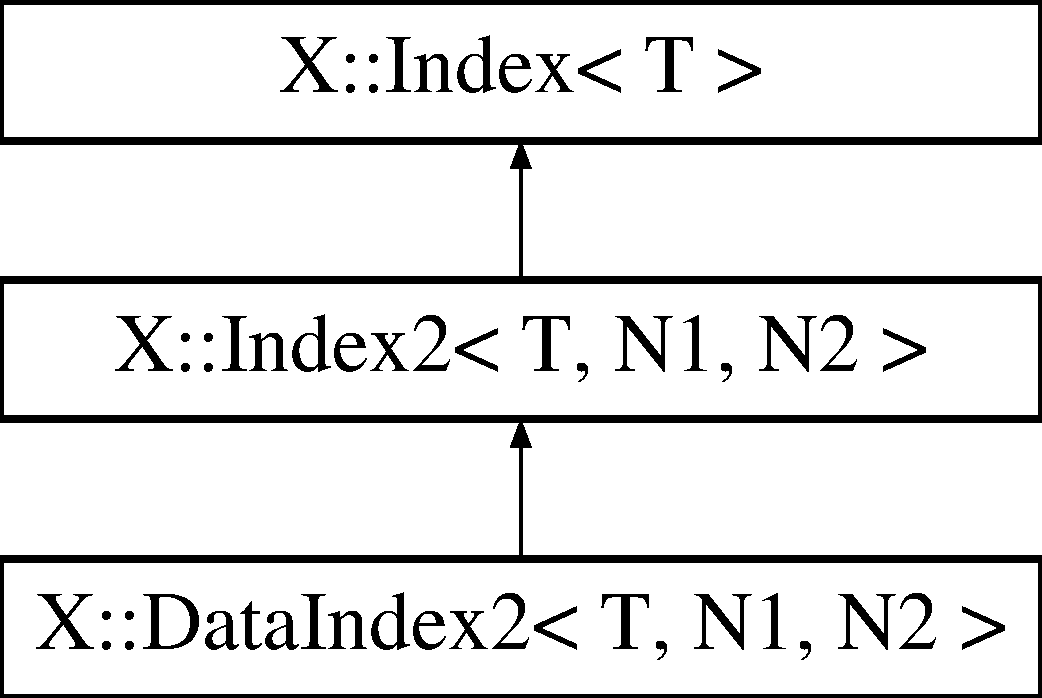
\includegraphics[height=3.000000cm]{class_x_1_1_index2}
\end{center}
\end{figure}
\subsection*{Public Member Functions}
\begin{DoxyCompactItemize}
\item 
\hypertarget{class_x_1_1_index2_a1b791266a385e8e171f4a1d5bc72e747}{{\bfseries Index2} (T $\ast$data)}\label{class_x_1_1_index2_a1b791266a385e8e171f4a1d5bc72e747}

\item 
\hypertarget{class_x_1_1_index2_a06e8ccdbe72125ccff7b5d8db35892e7}{virtual T \& {\bfseries operator()} (xsize i, xsize j)}\label{class_x_1_1_index2_a06e8ccdbe72125ccff7b5d8db35892e7}

\end{DoxyCompactItemize}
\subsubsection*{template$<$typename T, xsize N1, xsize N2$>$ class X\-::\-Index2$<$ T, N1, N2 $>$}



The documentation for this class was generated from the following file\-:\begin{DoxyCompactItemize}
\item 
src/index\-\_\-2.\-h\end{DoxyCompactItemize}

\hypertarget{class_x_1_1_matrix}{\section{X\-:\-:Matrix$<$ T, R\-O\-W\-S, C\-O\-L\-S $>$ Class Template Reference}
\label{class_x_1_1_matrix}\index{X\-::\-Matrix$<$ T, R\-O\-W\-S, C\-O\-L\-S $>$@{X\-::\-Matrix$<$ T, R\-O\-W\-S, C\-O\-L\-S $>$}}
}
\subsection*{Public Member Functions}
\begin{DoxyCompactItemize}
\item 
\hypertarget{class_x_1_1_matrix_ab75b1d2bc186c792b11626696cf2c47e}{{\bfseries Matrix} (T $\ast$data)}\label{class_x_1_1_matrix_ab75b1d2bc186c792b11626696cf2c47e}

\item 
\hypertarget{class_x_1_1_matrix_af8410e867fae9f62d5587a28122f1ace}{{\bfseries Matrix} (T init\-\_\-value)}\label{class_x_1_1_matrix_af8410e867fae9f62d5587a28122f1ace}

\item 
\hypertarget{class_x_1_1_matrix_aacd5faf4f5c633c6d54aeb656da0d743}{{\bfseries Matrix} (\hyperlink{class_x_1_1_matrix}{Matrix}$<$ T, R\-O\-W\-S, C\-O\-L\-S $>$ \&original)}\label{class_x_1_1_matrix_aacd5faf4f5c633c6d54aeb656da0d743}

\item 
\hypertarget{class_x_1_1_matrix_a9f1d9bd53f9e5c0c34e09cba0e11dc97}{void {\bfseries Default\-Constructor} ()}\label{class_x_1_1_matrix_a9f1d9bd53f9e5c0c34e09cba0e11dc97}

\item 
\hypertarget{class_x_1_1_matrix_a2e89dff425c5ed24a83758ab91d37c4d}{\hyperlink{class_x_1_1_matrix}{Matrix}$<$ T, R\-O\-W\-S, C\-O\-L\-S $>$ \& {\bfseries copy\-From} (\hyperlink{class_x_1_1_matrix}{Matrix}$<$ T, R\-O\-W\-S, C\-O\-L\-S $>$ \&mtx\-B)}\label{class_x_1_1_matrix_a2e89dff425c5ed24a83758ab91d37c4d}

\item 
\hypertarget{class_x_1_1_matrix_ab78d80b8ca8247ee02f34a8269fd54d1}{\hyperlink{class_x_1_1_matrix}{Matrix}$<$ T, R\-O\-W\-S, C\-O\-L\-S $>$ \& {\bfseries negate} ()}\label{class_x_1_1_matrix_ab78d80b8ca8247ee02f34a8269fd54d1}

\item 
\hypertarget{class_x_1_1_matrix_a19fe6c74400a6bd42ae7ee9e08aea35f}{\hyperlink{class_x_1_1_matrix}{Matrix}$<$ T, R\-O\-W\-S, C\-O\-L\-S $>$ \& {\bfseries reciprocal} ()}\label{class_x_1_1_matrix_a19fe6c74400a6bd42ae7ee9e08aea35f}

\item 
\hypertarget{class_x_1_1_matrix_a6497d0d19cfc10a59379688288c641c4}{\hyperlink{class_x_1_1_matrix}{Matrix}$<$ T, R\-O\-W\-S, C\-O\-L\-S $>$ \& {\bfseries each} (void($\ast$)(T)) const }\label{class_x_1_1_matrix_a6497d0d19cfc10a59379688288c641c4}

\item 
\hypertarget{class_x_1_1_matrix_af9ae720c5001887c594c775ec16c138b}{xsize {\bfseries get\-Elms} () const }\label{class_x_1_1_matrix_af9ae720c5001887c594c775ec16c138b}

\item 
\hypertarget{class_x_1_1_matrix_ac7819d8516e7b389990c6bc4fb9a3bc2}{xsize {\bfseries get\-Rows} () const }\label{class_x_1_1_matrix_ac7819d8516e7b389990c6bc4fb9a3bc2}

\item 
\hypertarget{class_x_1_1_matrix_a30ada40f567ef2c38eb1055553a03c90}{xsize {\bfseries get\-Cols} () const }\label{class_x_1_1_matrix_a30ada40f567ef2c38eb1055553a03c90}

\item 
\hypertarget{class_x_1_1_matrix_aed16c8b920e59640d90fbf17f604c32a}{T $\ast$ {\bfseries get\-Ptr} () const }\label{class_x_1_1_matrix_aed16c8b920e59640d90fbf17f604c32a}

\item 
\hypertarget{class_x_1_1_matrix_a4c1e4ea005aadc3198d4545031c279f6}{\hyperlink{class_x_1_1_matrix}{Matrix}$<$ T, R\-O\-W\-S, C\-O\-L\-S $>$ \& {\bfseries add\-By} (\hyperlink{class_x_1_1_matrix}{Matrix}$<$ T, R\-O\-W\-S, C\-O\-L\-S $>$ \&)}\label{class_x_1_1_matrix_a4c1e4ea005aadc3198d4545031c279f6}

\item 
\hypertarget{class_x_1_1_matrix_a1b012fbcad54bc01d6a40b1aa7dd7dc6}{\hyperlink{class_x_1_1_matrix}{Matrix}$<$ T, R\-O\-W\-S, C\-O\-L\-S $>$ \& {\bfseries sub\-By} (\hyperlink{class_x_1_1_matrix}{Matrix}$<$ T, R\-O\-W\-S, C\-O\-L\-S $>$ \&)}\label{class_x_1_1_matrix_a1b012fbcad54bc01d6a40b1aa7dd7dc6}

\item 
\hypertarget{class_x_1_1_matrix_a4e8a7db49b11b2362149176accff6ae1}{\hyperlink{class_x_1_1_matrix}{Matrix}$<$ T, R\-O\-W\-S, C\-O\-L\-S $>$ \& {\bfseries mul\-By} (\hyperlink{class_x_1_1_matrix}{Matrix}$<$ T, R\-O\-W\-S, C\-O\-L\-S $>$ \&)}\label{class_x_1_1_matrix_a4e8a7db49b11b2362149176accff6ae1}

\item 
\hypertarget{class_x_1_1_matrix_a5f7f50bbcc5724cb38042b9016c468df}{\hyperlink{class_x_1_1_matrix}{Matrix}$<$ T, R\-O\-W\-S, C\-O\-L\-S $>$ \& {\bfseries div\-By} (\hyperlink{class_x_1_1_matrix}{Matrix}$<$ T, R\-O\-W\-S, C\-O\-L\-S $>$ \&)}\label{class_x_1_1_matrix_a5f7f50bbcc5724cb38042b9016c468df}

\item 
\hypertarget{class_x_1_1_matrix_a4c4a84b225a3aef48dc2e290a801a42c}{\hyperlink{class_x_1_1_matrix}{Matrix}$<$ T, R\-O\-W\-S, C\-O\-L\-S $>$ \& {\bfseries add\-By} (T)}\label{class_x_1_1_matrix_a4c4a84b225a3aef48dc2e290a801a42c}

\item 
\hypertarget{class_x_1_1_matrix_a128686e35d3b3b56615472248d152f9a}{\hyperlink{class_x_1_1_matrix}{Matrix}$<$ T, R\-O\-W\-S, C\-O\-L\-S $>$ \& {\bfseries sub\-By} (T)}\label{class_x_1_1_matrix_a128686e35d3b3b56615472248d152f9a}

\item 
\hypertarget{class_x_1_1_matrix_a4a93e65e99ade587f47d604375336f81}{\hyperlink{class_x_1_1_matrix}{Matrix}$<$ T, R\-O\-W\-S, C\-O\-L\-S $>$ \& {\bfseries mul\-By} (T)}\label{class_x_1_1_matrix_a4a93e65e99ade587f47d604375336f81}

\item 
\hypertarget{class_x_1_1_matrix_a5f07640d5fc4c9ec5d8984e66e4b1b04}{\hyperlink{class_x_1_1_matrix}{Matrix}$<$ T, R\-O\-W\-S, C\-O\-L\-S $>$ \& {\bfseries div\-By} (T)}\label{class_x_1_1_matrix_a5f07640d5fc4c9ec5d8984e66e4b1b04}

\item 
\hypertarget{class_x_1_1_matrix_a3f53a8c894100f5a866cc3f5cfe905ee}{\hyperlink{class_x_1_1_matrix}{Matrix}$<$ T, R\-O\-W\-S, C\-O\-L\-S $>$ \& {\bfseries add\-Of} (\hyperlink{class_x_1_1_matrix}{Matrix}$<$ T, R\-O\-W\-S, C\-O\-L\-S $>$ \&, \hyperlink{class_x_1_1_matrix}{Matrix}$<$ T, R\-O\-W\-S, C\-O\-L\-S $>$ \&)}\label{class_x_1_1_matrix_a3f53a8c894100f5a866cc3f5cfe905ee}

\item 
\hypertarget{class_x_1_1_matrix_a3fd0ef2782f53565818707c98955a928}{\hyperlink{class_x_1_1_matrix}{Matrix}$<$ T, R\-O\-W\-S, C\-O\-L\-S $>$ \& {\bfseries sub\-Of} (\hyperlink{class_x_1_1_matrix}{Matrix}$<$ T, R\-O\-W\-S, C\-O\-L\-S $>$ \&, \hyperlink{class_x_1_1_matrix}{Matrix}$<$ T, R\-O\-W\-S, C\-O\-L\-S $>$ \&)}\label{class_x_1_1_matrix_a3fd0ef2782f53565818707c98955a928}

\item 
\hypertarget{class_x_1_1_matrix_a435b57c5d96ba16c44b60a3d23a9935f}{\hyperlink{class_x_1_1_matrix}{Matrix}$<$ T, R\-O\-W\-S, C\-O\-L\-S $>$ \& {\bfseries mul\-Of} (\hyperlink{class_x_1_1_matrix}{Matrix}$<$ T, R\-O\-W\-S, C\-O\-L\-S $>$ \&, \hyperlink{class_x_1_1_matrix}{Matrix}$<$ T, R\-O\-W\-S, C\-O\-L\-S $>$ \&)}\label{class_x_1_1_matrix_a435b57c5d96ba16c44b60a3d23a9935f}

\item 
\hypertarget{class_x_1_1_matrix_ab1f3e5c669f7584b16055913cb4f538f}{\hyperlink{class_x_1_1_matrix}{Matrix}$<$ T, R\-O\-W\-S, C\-O\-L\-S $>$ \& {\bfseries div\-Of} (\hyperlink{class_x_1_1_matrix}{Matrix}$<$ T, R\-O\-W\-S, C\-O\-L\-S $>$ \&, \hyperlink{class_x_1_1_matrix}{Matrix}$<$ T, R\-O\-W\-S, C\-O\-L\-S $>$ \&)}\label{class_x_1_1_matrix_ab1f3e5c669f7584b16055913cb4f538f}

\item 
\hypertarget{class_x_1_1_matrix_a8c18d62993f71d59fecf1d359a74021d}{\hyperlink{class_x_1_1_matrix}{Matrix}$<$ T, R\-O\-W\-S, C\-O\-L\-S $>$ \& {\bfseries add\-Of} (T, \hyperlink{class_x_1_1_matrix}{Matrix}$<$ T, R\-O\-W\-S, C\-O\-L\-S $>$ \&)}\label{class_x_1_1_matrix_a8c18d62993f71d59fecf1d359a74021d}

\item 
\hypertarget{class_x_1_1_matrix_addacb32638af825647a6b4f2952f1d68}{\hyperlink{class_x_1_1_matrix}{Matrix}$<$ T, R\-O\-W\-S, C\-O\-L\-S $>$ \& {\bfseries sub\-Of} (T, \hyperlink{class_x_1_1_matrix}{Matrix}$<$ T, R\-O\-W\-S, C\-O\-L\-S $>$ \&)}\label{class_x_1_1_matrix_addacb32638af825647a6b4f2952f1d68}

\item 
\hypertarget{class_x_1_1_matrix_a6da2d4a1604d164b402fd728c2df1e2a}{\hyperlink{class_x_1_1_matrix}{Matrix}$<$ T, R\-O\-W\-S, C\-O\-L\-S $>$ \& {\bfseries mul\-Of} (T, \hyperlink{class_x_1_1_matrix}{Matrix}$<$ T, R\-O\-W\-S, C\-O\-L\-S $>$ \&)}\label{class_x_1_1_matrix_a6da2d4a1604d164b402fd728c2df1e2a}

\item 
\hypertarget{class_x_1_1_matrix_a1e795cd35cc4fc12915fd1c9c6eafa49}{\hyperlink{class_x_1_1_matrix}{Matrix}$<$ T, R\-O\-W\-S, C\-O\-L\-S $>$ \& {\bfseries div\-Of} (T, \hyperlink{class_x_1_1_matrix}{Matrix}$<$ T, R\-O\-W\-S, C\-O\-L\-S $>$ \&)}\label{class_x_1_1_matrix_a1e795cd35cc4fc12915fd1c9c6eafa49}

\item 
\hypertarget{class_x_1_1_matrix_a7d1617d11137b067ebff88066a6a93ef}{\hyperlink{class_x_1_1_matrix}{Matrix}$<$ T, R\-O\-W\-S, C\-O\-L\-S $>$ \& {\bfseries add\-Of} (\hyperlink{class_x_1_1_matrix}{Matrix}$<$ T, R\-O\-W\-S, C\-O\-L\-S $>$ \&, T)}\label{class_x_1_1_matrix_a7d1617d11137b067ebff88066a6a93ef}

\item 
\hypertarget{class_x_1_1_matrix_a4d2ba824caff2cc99c2c024d4714f54f}{\hyperlink{class_x_1_1_matrix}{Matrix}$<$ T, R\-O\-W\-S, C\-O\-L\-S $>$ \& {\bfseries sub\-Of} (\hyperlink{class_x_1_1_matrix}{Matrix}$<$ T, R\-O\-W\-S, C\-O\-L\-S $>$ \&, T)}\label{class_x_1_1_matrix_a4d2ba824caff2cc99c2c024d4714f54f}

\item 
\hypertarget{class_x_1_1_matrix_a1ca2d2fc417228449b500e583c89c194}{\hyperlink{class_x_1_1_matrix}{Matrix}$<$ T, R\-O\-W\-S, C\-O\-L\-S $>$ \& {\bfseries mul\-Of} (\hyperlink{class_x_1_1_matrix}{Matrix}$<$ T, R\-O\-W\-S, C\-O\-L\-S $>$ \&, T)}\label{class_x_1_1_matrix_a1ca2d2fc417228449b500e583c89c194}

\item 
\hypertarget{class_x_1_1_matrix_a3827f511425bccd9d6fcdfffea305380}{\hyperlink{class_x_1_1_matrix}{Matrix}$<$ T, R\-O\-W\-S, C\-O\-L\-S $>$ \& {\bfseries div\-Of} (\hyperlink{class_x_1_1_matrix}{Matrix}$<$ T, R\-O\-W\-S, C\-O\-L\-S $>$ \&, T)}\label{class_x_1_1_matrix_a3827f511425bccd9d6fcdfffea305380}

\item 
\hypertarget{class_x_1_1_matrix_ac2a654d2319a0be6386c380662972c1a}{void {\bfseries reset\-Offset} ()}\label{class_x_1_1_matrix_ac2a654d2319a0be6386c380662972c1a}

\item 
\hypertarget{class_x_1_1_matrix_ad98787fc46e620922f8f663cd311a4f5}{void {\bfseries set\-Offset} (xsize offset)}\label{class_x_1_1_matrix_ad98787fc46e620922f8f663cd311a4f5}

\item 
\hypertarget{class_x_1_1_matrix_abf02b1c525d47e389dcb14679f51c84f}{xsize {\bfseries get\-Offset} () const }\label{class_x_1_1_matrix_abf02b1c525d47e389dcb14679f51c84f}

\item 
\hypertarget{class_x_1_1_matrix_a869186f779e32a8324c439307215d2c9}{\hyperlink{class_x_1_1_matrix}{Matrix}$<$ T, R\-O\-W\-S, C\-O\-L\-S $>$ \& {\bfseries operator=} (\hyperlink{class_x_1_1_matrix}{Matrix}$<$ T, R\-O\-W\-S, C\-O\-L\-S $>$ \&)}\label{class_x_1_1_matrix_a869186f779e32a8324c439307215d2c9}

\item 
\hypertarget{class_x_1_1_matrix_ad2953fafd8758c9c3c79e5c7607aad37}{T \& {\bfseries operator()} (xsize)}\label{class_x_1_1_matrix_ad2953fafd8758c9c3c79e5c7607aad37}

\item 
\hypertarget{class_x_1_1_matrix_a1048d1369ba7ae4d4e0dec4200523ee4}{T \& {\bfseries operator()} (xsize, xsize)}\label{class_x_1_1_matrix_a1048d1369ba7ae4d4e0dec4200523ee4}

\item 
\hypertarget{class_x_1_1_matrix_aab9d681351a2873e830d3cf0226a256b}{\hyperlink{class_x_1_1_matrix}{Matrix}$<$ T, R\-O\-W\-S, C\-O\-L\-S $>$ \& {\bfseries operator$<$$<$} (T)}\label{class_x_1_1_matrix_aab9d681351a2873e830d3cf0226a256b}

\item 
\hypertarget{class_x_1_1_matrix_ae91830bdce6c3c7cd5433be007765700}{\hyperlink{class_x_1_1_matrix}{Matrix}$<$ T, R\-O\-W\-S, C\-O\-L\-S $>$ \& {\bfseries operator,} (T)}\label{class_x_1_1_matrix_ae91830bdce6c3c7cd5433be007765700}

\end{DoxyCompactItemize}
\subsubsection*{template$<$typename T, xsize R\-O\-W\-S, xsize C\-O\-L\-S$>$ class X\-::\-Matrix$<$ T, R\-O\-W\-S, C\-O\-L\-S $>$}



The documentation for this class was generated from the following file\-:\begin{DoxyCompactItemize}
\item 
src/matrix.\-h\end{DoxyCompactItemize}

\hypertarget{class_x_1_1_memory}{\section{X\-:\-:Memory Class Reference}
\label{class_x_1_1_memory}\index{X\-::\-Memory@{X\-::\-Memory}}
}
\subsection*{Static Public Member Functions}
\begin{DoxyCompactItemize}
\item 
\hypertarget{class_x_1_1_memory_ad4c4cb43672d7ab7f2543e68cd40b93a}{static void $\ast$ {\bfseries memory\-\_\-alloc} (unsigned int num\-\_\-of\-\_\-bytes)}\label{class_x_1_1_memory_ad4c4cb43672d7ab7f2543e68cd40b93a}

\item 
\hypertarget{class_x_1_1_memory_a2eef9505ead1adcba03628665c025ed6}{static void {\bfseries add\-\_\-pointer} (void $\ast$p)}\label{class_x_1_1_memory_a2eef9505ead1adcba03628665c025ed6}

\item 
\hypertarget{class_x_1_1_memory_ad866f58377ffede78835829f6574541b}{static void {\bfseries memory\-\_\-free\-\_\-all} ()}\label{class_x_1_1_memory_ad866f58377ffede78835829f6574541b}

\item 
\hypertarget{class_x_1_1_memory_a53866b5281569781abeb525035554681}{static void {\bfseries memory\-\_\-free} (void $\ast$p)}\label{class_x_1_1_memory_a53866b5281569781abeb525035554681}

\end{DoxyCompactItemize}


The documentation for this class was generated from the following file\-:\begin{DoxyCompactItemize}
\item 
src/memory.\-h\end{DoxyCompactItemize}

\hypertarget{class_x_1_1_meshgrid_field2_filestream}{\section{X\-:\-:Meshgrid\-Field2\-Filestream$<$ T, P1, P2, N $>$ Class Template Reference}
\label{class_x_1_1_meshgrid_field2_filestream}\index{X\-::\-Meshgrid\-Field2\-Filestream$<$ T, P1, P2, N $>$@{X\-::\-Meshgrid\-Field2\-Filestream$<$ T, P1, P2, N $>$}}
}
\subsubsection*{template$<$typename T, xsize P1, xsize P2, xsize N$>$ class X\-::\-Meshgrid\-Field2\-Filestream$<$ T, P1, P2, N $>$}



The documentation for this class was generated from the following file\-:\begin{DoxyCompactItemize}
\item 
src/filestream.\-h\end{DoxyCompactItemize}

\hypertarget{class_normal_operation_3_01typename_01_t_00_01xsize_01_n_01_4}{\section{Normal\-Operation$<$ typename T, xsize N $>$ Class Reference}
\label{class_normal_operation_3_01typename_01_t_00_01xsize_01_n_01_4}\index{Normal\-Operation$<$ typename T, xsize N $>$@{Normal\-Operation$<$ typename T, xsize N $>$}}
}


The documentation for this class was generated from the following file\-:\begin{DoxyCompactItemize}
\item 
src/normal\-\_\-operation.\-h\end{DoxyCompactItemize}

\hypertarget{class_x_1_1_vector}{\section{X\-:\-:Vector$<$ T, N $>$ Class Template Reference}
\label{class_x_1_1_vector}\index{X\-::\-Vector$<$ T, N $>$@{X\-::\-Vector$<$ T, N $>$}}
}
Inheritance diagram for X\-:\-:Vector$<$ T, N $>$\-:\begin{figure}[H]
\begin{center}
\leavevmode
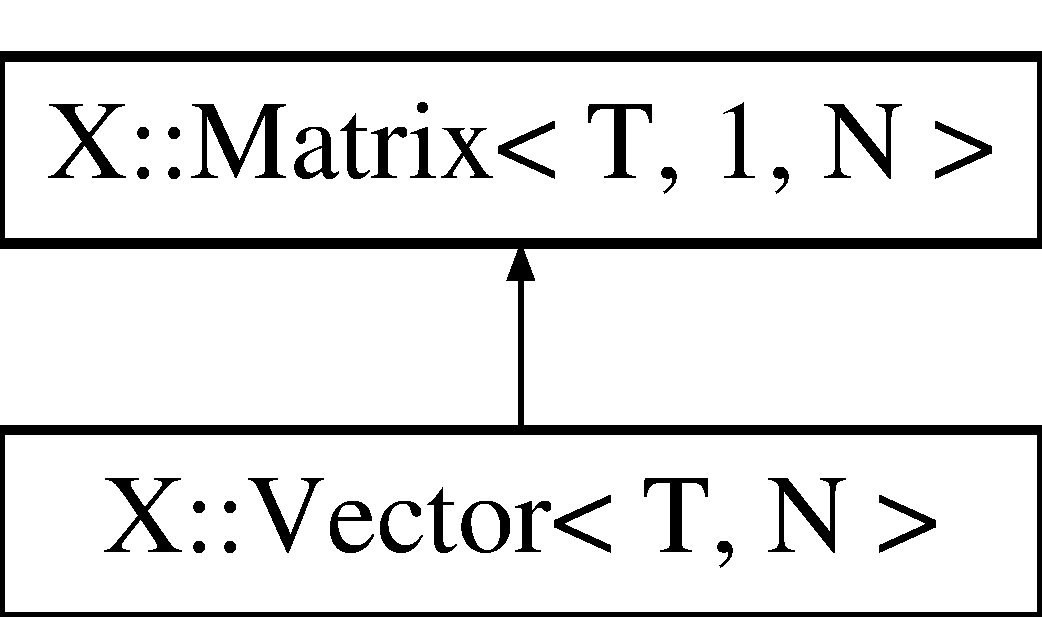
\includegraphics[height=2.000000cm]{class_x_1_1_vector}
\end{center}
\end{figure}
\subsection*{Public Member Functions}
\begin{DoxyCompactItemize}
\item 
\hypertarget{class_x_1_1_vector_a8ab40898cfe1b88e72eb65fdbf02e65c}{{\bfseries Vector} (T $\ast$data)}\label{class_x_1_1_vector_a8ab40898cfe1b88e72eb65fdbf02e65c}

\item 
\hypertarget{class_x_1_1_vector_a957893ba7708b81325d1815622f25f11}{{\bfseries Vector} (T init\-\_\-value)}\label{class_x_1_1_vector_a957893ba7708b81325d1815622f25f11}

\item 
\hypertarget{class_x_1_1_vector_ac5e9e3616cbd335f51d78f414d90b73d}{{\bfseries Vector} (\hyperlink{class_x_1_1_vector}{Vector}$<$ T, N $>$ \&original)}\label{class_x_1_1_vector_ac5e9e3616cbd335f51d78f414d90b73d}

\item 
\hypertarget{class_x_1_1_vector_a10325386231775ef382c19a413f45cb6}{T $\ast$ {\bfseries get\-Ptr} ()}\label{class_x_1_1_vector_a10325386231775ef382c19a413f45cb6}

\end{DoxyCompactItemize}
\subsubsection*{template$<$typename T, xsize N$>$ class X\-::\-Vector$<$ T, N $>$}



The documentation for this class was generated from the following file\-:\begin{DoxyCompactItemize}
\item 
src/vector.\-h\end{DoxyCompactItemize}

\hypertarget{class_x_1_1x_complex}{\section{X\-:\-:x\-Complex$<$ T $>$ Class Template Reference}
\label{class_x_1_1x_complex}\index{X\-::x\-Complex$<$ T $>$@{X\-::x\-Complex$<$ T $>$}}
}
\subsubsection*{template$<$typename T$>$ class X\-::x\-Complex$<$ T $>$}



The documentation for this class was generated from the following file\-:\begin{DoxyCompactItemize}
\item 
src/xcomplex.\-h\end{DoxyCompactItemize}

\printindex
\end{document}
